\section{壹、前言}

\subsection{一、研究動機}

近年來,物件追蹤技術被廣泛應用於球類運動上,例如鷹眼系統(Hawk-Eye)已被應用於網球、羽球等運動,以追蹤和記錄球的路徑。然而由於其架設成本高,多數運動員無法負擔。為了解決此問題,國立交通大學網路最佳化實驗室開發了深度學習架構 TrackNet,可以由一般攝影機拍攝之網球比賽影片追蹤網球軌跡。(鍾奉原,2020)

排球在我校是非常興盛的一種運動,經常舉辦班際球賽等排球比賽,因此我們便想利用 TrackNetV2 追蹤排球比賽影片中的排球,以協助分析排球比賽,減少人工花費大量時間觀看的成本。

\subsection{二、研究目的}

應用 TrackNetV2 追蹤由一般攝影機(非高速攝影機)所錄製之排球比賽影片中的排球,藉由自動追蹤球的路徑協助排球比賽的賽事分析。

\subsection{三、文獻回顧}

傳統影像物件辨識是根據物件的外顯特徵和統計特徵進行偵測的,但排球比賽中的排球會因打擊的關係而導致有變形的情況出現,再加上移動速度過快,快門相對於球的速度來說較慢,因此容易有影像殘留及模糊的現象出現。

\begin{itemize}
    \setlength\parindent{2em}
    \item []
    \textbf{(一)TrackNet}

    TrackNet(黃昱銓,2018)提出了一個以 CNN(Convolutional Neural Network,卷積神經網路)為基礎的深度學習架構(如圖 \ref{TrackNet 架構圖})。但不同於其他深度學習網路,它容許一次輸入多張連續幀,可從中學習球的影像特徵及軌跡特性。然後仿效 FCN(Fully Convolutional Network,全卷積網路)的生成階段,生成用於偵測及定位球的熱度圖(如圖 \ref{熱度圖})。最後再依據熱度圖計算畫面中可能存在的網球。這個模型不僅能從模糊影像中定位球的存在,更可以進一步的判斷受遮擋的網球位置,可以很好的達到我們的需求。
    
    \begin{figure}[H]
        \centering
        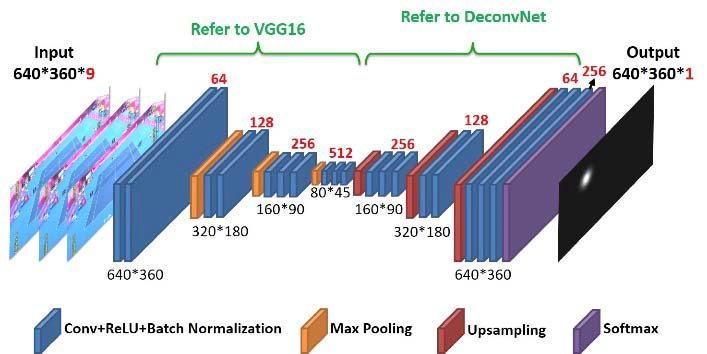
\includegraphics[width = 9cm]{picture/TrackNet 架構圖.jpg}\\
        \caption{、TrackNet 架構圖(黃昱銓,2018)}
        \label{TrackNet 架構圖}
        \vspace{1cm}
        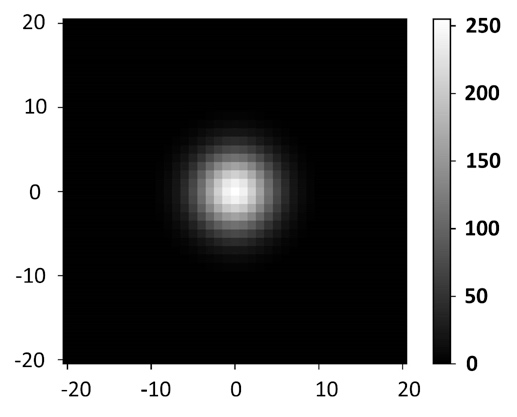
\includegraphics[width = 7cm]{picture/熱度圖.jpg}
        \caption{、熱度圖(黃昱銓,2018)}
        \label{熱度圖}
    \end{figure}
    \item []
    \textbf{(二)TrackNetV2}

    TrackNetV2(Nian-En Sun et al., 2020)在 TrackNet 的基礎上改進了它的處理速度、準確度、記憶體用量等。他們將 TrackNet 的模型重新設計,讓它從一個 MISO(Multiple-In Single-Out)的模型變成一個 MIMO(Multiple-In Multiple-Out)的模型,處理速度從原本的 2.6 FPS(Frame per second)上升到 31.8 FPS。他們也參考了 U-Net 的 skip connection(殘差連接),將卷積層所得的特徵圖(feature map)串聯到相應的上採樣層(upsampling layer),以此方式將低層次與高層次的特徵結合起來以提高準確度。他們所使用的資料集為來自 18 場羽球比賽共 55563 幀的羽球比賽影片。

    \begin{figure}[H]
        \centering
        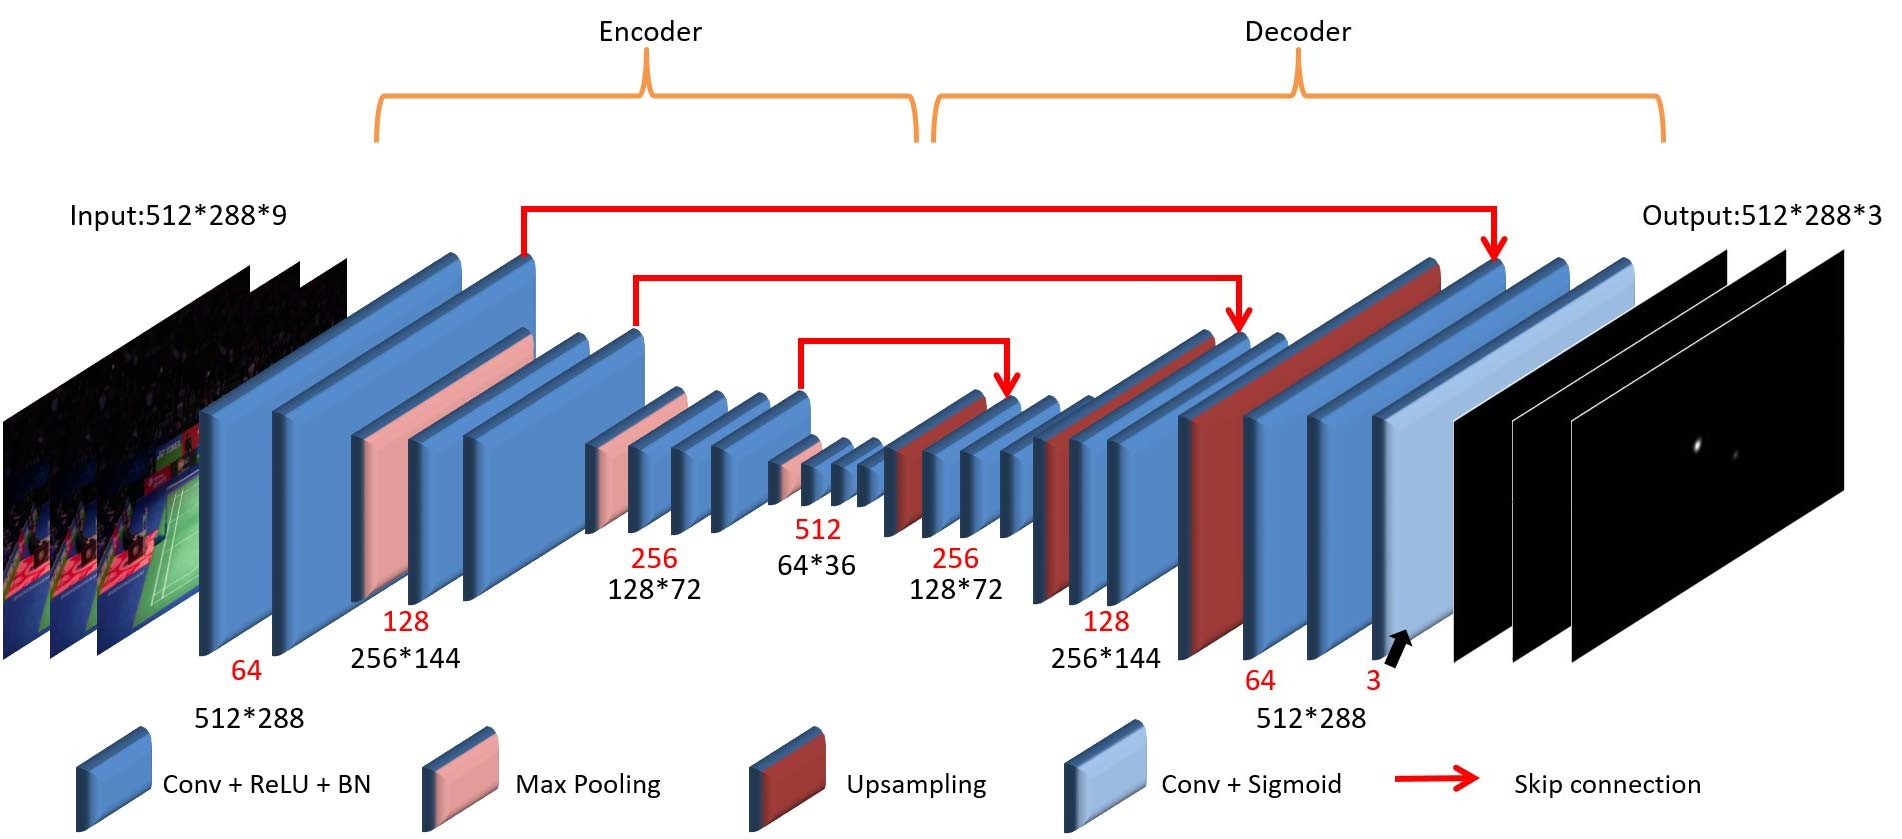
\includegraphics[width = 9cm]{picture/TrackNetV2 架構圖.jpg}
        \caption{、TrackNetV2 架構圖(Nian-En Sun et al., 2020)}
        \label{TrackNetV2 架構圖}
    \end{figure}

    \item []
    \textbf{(三)卷積神經網路}

    卷積神經網路(Convolutional Neural Network, CNN)是一種深度學習的神經網路模型,常被應用於影像識別方面。CNN 的結構包含卷積層(Convolution Layer)、池化層(Pooling Layer)、全連接層(Fully Connected Layer)。

    \begin{itemize}
        \setlength\parindent{2em}
        \item []
        \textbf{1. 概念}

        \begin{itemize}
            \setlength\parindent{2em}
            \item []
            \textbf{(1)權值共享}

            在一般的圖像內有許多的特徵是相同的,如特定的輪廓或線條,那我們就可以讓相同幾個神經元組成的卷積核去學習這個特徵,透過滑動窗口對整張圖片進行卷積,進而達到節省參數的效果。(Cinnamon AI Taiwan,2019)

            \item []
            \textbf{(2)保留位置資訊}

            圖片中的像素(Pixels)與其鄰近的像素會有一定的關聯度,若使用 FC(Fully Connected,全連接網路結構)的結構來訓練圖像資訊的話,要先通過一個展開(Flatten)的步驟,把高維的資訊拉成一條直線,如此一來就會大量失去特徵之間的空間資訊。(Cinnamon AI Taiwan,2019)
        \end{itemize}

        \item []
        \textbf{2. 結構}

        \begin{itemize}
            \setlength\parindent{2em}
            \item []
            \textbf{(1)卷積層(Convolution Layer)}

            卷積層負責提取圖像中的局部特徵,其原理是透過許多的卷積核(kernel)在圖片上進行滑動擷取特徵。將圖片與特定的卷積核進行卷積運算。

            \begin{figure}[H]
                \centering
                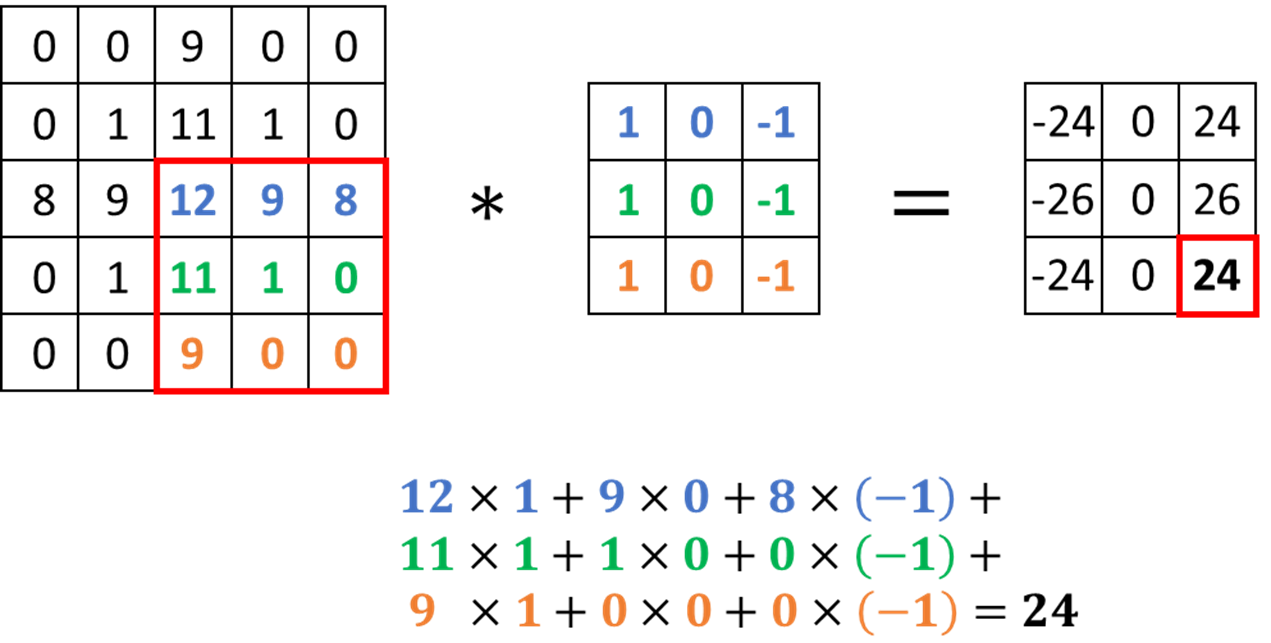
\includegraphics[width = 9cm]{picture/卷積層.jpg}
                \caption{、卷積層(Brandon Da Silva,2018)}
                \label{卷積層}
            \end{figure}

            \item []
            \textbf{(2)池化層(Pooling Layer)}

            池化層是用來大幅降低參數量級(降維)、降低過擬合問題、緩解卷積層對位置的敏感度。池化層的計算與卷積層一樣,都是透過滑動視窗框選的局部數值進行數值運算,最常用的計算方式為 Max pooling,在框選的局部數值中挑出最大值。(李謦伊,2020)
        
            \begin{figure}[H]
                \centering
                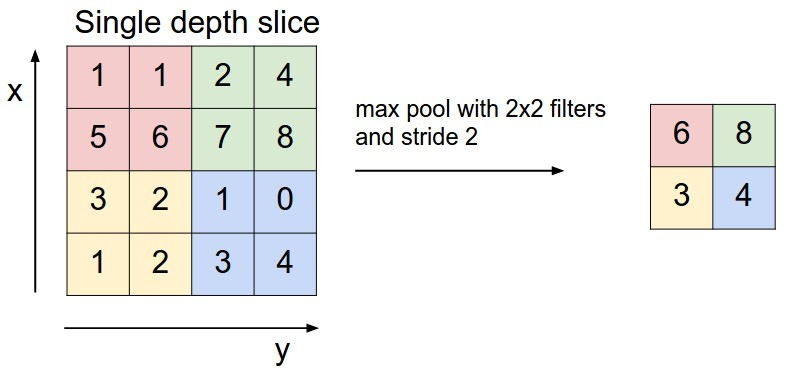
\includegraphics[width = 9cm]{picture/池化層.jpg}
                \caption{、池化層(Max pooling)(cs231n,2021)}
                \label{池化層}
            \end{figure}

            \item []
            \textbf{(3)全連接層(Fully Connected Layer)}

            在經過攤平(Flatten)變為一維數據後,全連接層(FC)主要在做最後的特徵提取,並且利用最後一層 FC 當作分類器。

        \end{itemize}
    \end{itemize}
\end{itemize}

\section{貳、研究設備與器材}

\subsection{一、硬體設備}

\begin{itemize}[itemindent = 2em]
    \item [(一)]中央處理器(CPU) AMD Ryzen 9 5950X 16-Core Processor
    \item [(二)]記憶體:32GiB
    \item [(三)]圖形處理器 (GPU):NVIDIA GeForce RTX 3090 (GPU 記憶體 24 GiB)
    \item [(四)]作業系統:Linux (Ubuntu 20.04.01)
\end{itemize}

\subsection{二、軟體及工具環境}

\begin{itemize}[itemindent = 2em]
    \item [(一)]Python 3.7.13:具有高效能的高階資料結構,直譯式且物件導向的程式語言。
    \item [(二)]moviepy.editor 1.0.3:是一個 Python 用來編輯影片的函式庫。
    \item [(三)]PyQt5 5.15.7:是一個 Python 用來創建圖形使用介面(Graphical User Interface, GUI)應用程式的函式庫。
    \item [(四)]pandas 1.3.5:是一個 Python 用來操作及分析資料的函式庫。
    \item [(五)]PyMySQL 1.0.2:是 Python 用來連接到 MySQL 資料庫伺服器的一個介面。
    \item [(六)]opencv-python 4.6.0.66:是一個用於解決電腦視覺相關問題的 Python 函式庫。
    \item [(七)]imutils 0.5.4:整合了 OpenCV 、 numpy 和 matplotlib 的相關操作的套件,主要用於進行圖像處理。
    \item [(八)]Pillow 9.2.0:是一個 Python 中用於影像辨識的套件庫,可以用來旋轉照片、嵌字、合成照片、變更圖片解析度等。
    \item [(九)]piexif 1.1.3:可以讀取與修改圖片 Exif(可交換圖檔格式)的套件,通常與 Pillow 搭配使用。
    \item [(十)]scikit-learn 1.0.2:是一個開源資料分析函式庫,具有各種分類、回歸和集群分析。
    \item [(十一)]keras 2.9.0:是一款用 Python 編寫而成的開源神經網路函式庫,能搭配 TensorFlow 、 Theano 等運作。
    \item [(十二)]TensorFlow 2.9.2:是現在重要的深度學習框架之一,支援各式不同的深度學習演算法。
    \item [(十三)]CUDA 10.1.243:是用於圖形處理單元(graphical processing units,GPU)的平行運算平台和程式設計模型。
\end{itemize}

\section{參、研究過程或方法}

\subsection{一、研究構思與架構}
\begin{figure}[H]
    \centering
    \begin{tikzpicture}[node distance=15pt]
        \node[box] (start) {閱讀相關文獻};
        \node[box, below = of start] (step 1) {使用 TrackNetV2 提供之資料集嘗試進行訓練};
        \node[box, below = of step 1] (step 2) {資料集收集};
        \node[box, below = of step 2] (step 3) {標記資料集};
        \node[box, below = of step 3] (step 4) {生成訓練數據};
        \node[box, below = of step 4] (step 5) {訓練模型};
        \node[box, below = of step 5] (step 6) {生成預測資料};
        \node[box, below = of step 6] (end) {效能評估};
        
        \graph {
            (start) -> (step 1) -> (step 2) -> (step 3) -> (step 4) -> (step 5) -> (step 6) -> (end);
        };
    \end{tikzpicture}
    \caption{、研究流程圖}
    \label{研究流程圖}
\end{figure}

圖 \ref{研究流程圖} 為我們的研究流程圖。首先我們閱讀 TrackNet、TrackNetV2 及其他物件追蹤相關論文,以了解相關技術,並嘗試使用 TrackNetV2 所提供的羽球資料集進行訓練,熟悉訓練流程並修改部分因版本更新無法使用的程式碼。

接下來我們由網路下載排球比賽影片,切割成「發球~死球」的數個影片,利用 Labeling Tool 標記排球中心在每幀的所在位置,然後生成熱度圖等訓練數據後進行訓練,最後由其他比賽擷取測試資料進行測試並評估性能。

\begin{table}[H]
    \centering
    \caption{、訓練集與測試集整理}
    \label{訓練集與測試集整理}
    \begin{tabular}{cccc}
        \hline
        \textbf{集別} & \textbf{比賽名稱} & \textbf{擷取長度} & \textbf{功能}\\
        \hline
        訓練集 & \makecell[c]{108UVL 大專排球聯賽女一級\\季軍賽} & 1240 秒 & \makecell[c]{人工標記排球位置後\\作為訓練資料訓練模型}\\
        \hline
        測試集 & \makecell[c]{108UVL 大專排球聯賽女一級\\冠軍賽} & 76 秒 & \makecell[c]{模型訓練完成後\\使用此測試資料測試模型性能}\\
        \hline
    \end{tabular}
\end{table}

\subsection{二、研究過程}

\begin{itemize}
    \setlength\parindent{2em}
    \item []
    \textbf{(一)資料集收集}

    我們由 108UVL 大專排球聯賽女一級季軍賽擷取比賽片段,為去除與`排球追蹤無關部分,每段子影片擷取發球到死球的段落,影片名稱為「局數\_A方比數\_B方比數」,如 1\_00\_00.mp4。影片幀數為每秒 30 幀,解析度為 $1920\times1080$。

    原影片長度 2 小時 14 分 35 秒,擷取後資料集全長共 1240 秒,37200 幀。

    \begin{figure}[H]
        \centering
        \begin{minipage}[t]{0.48\textwidth}
            \centering
            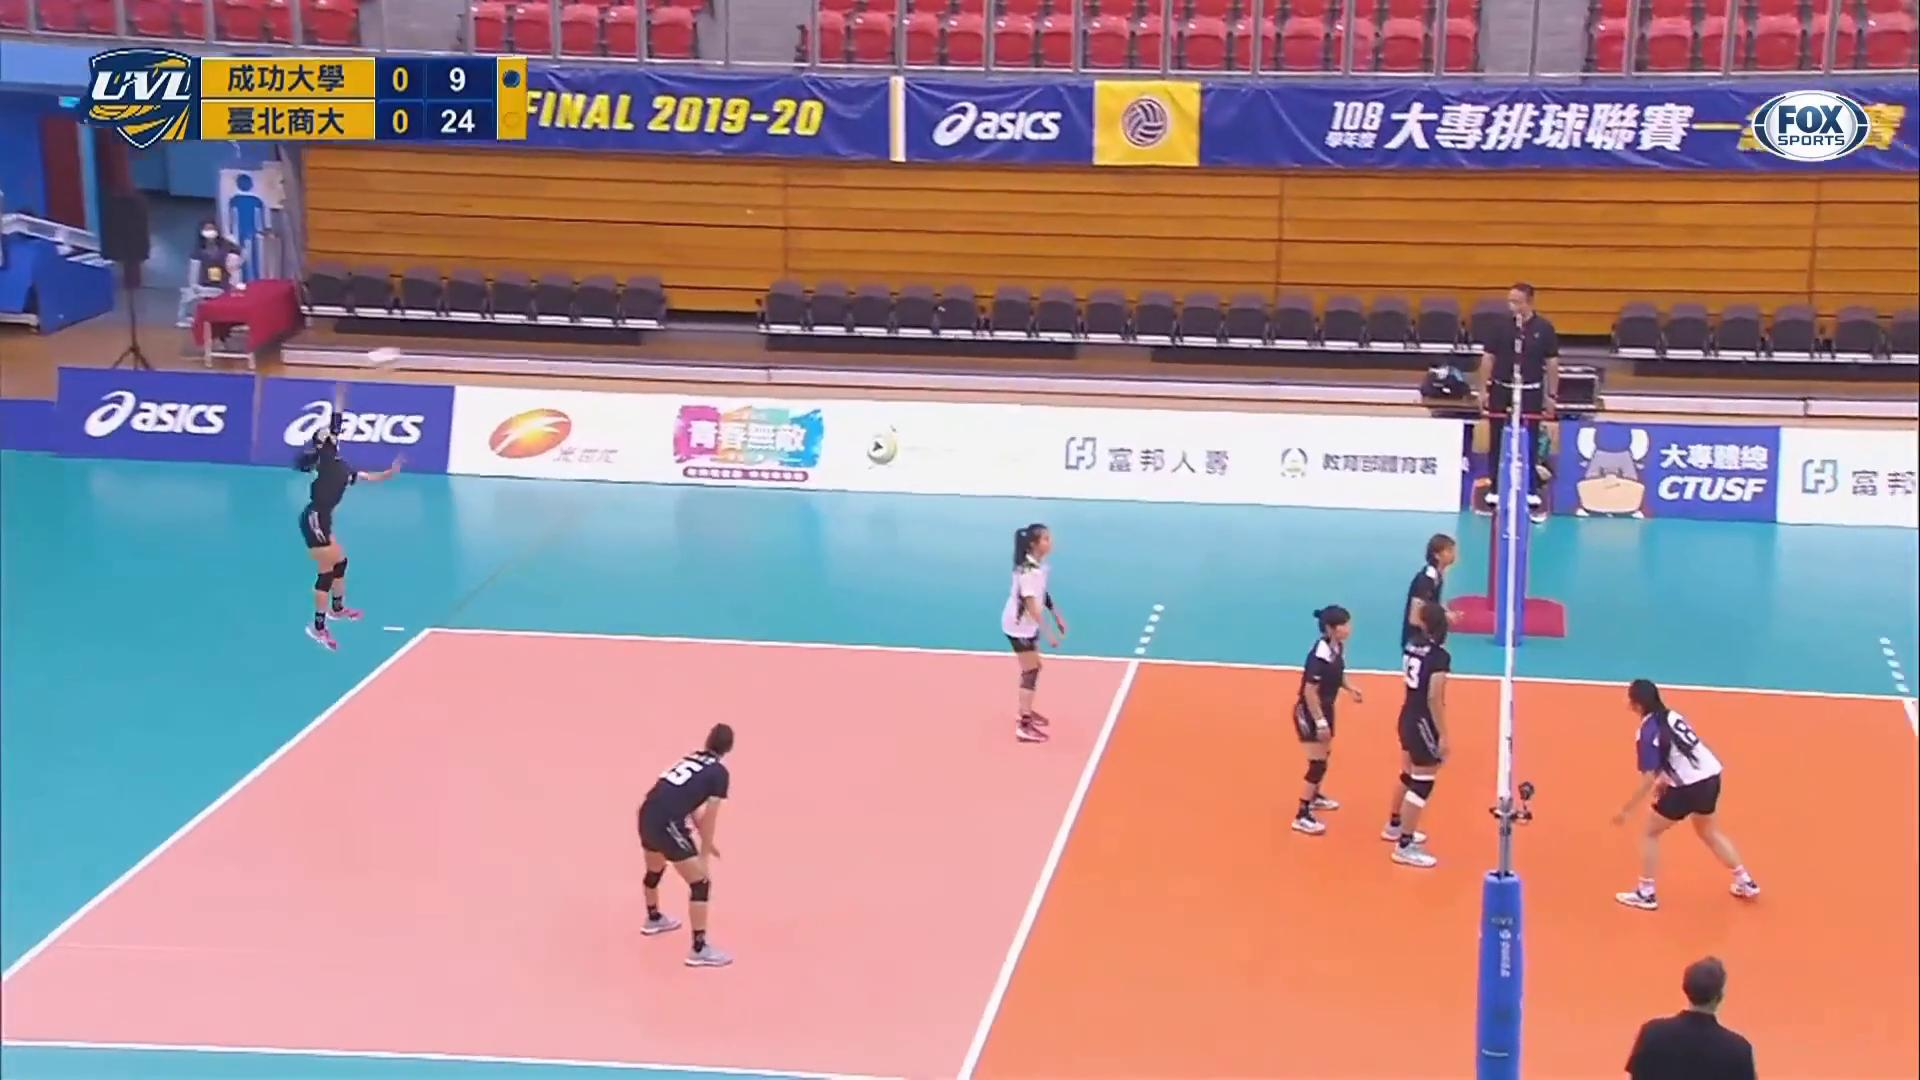
\includegraphics[width = 7cm]{picture/發球.jpg}
            \caption{、發球}
            \label{發球}
        \end{minipage}
        \begin{minipage}[t]{0.48\textwidth}
            \centering
            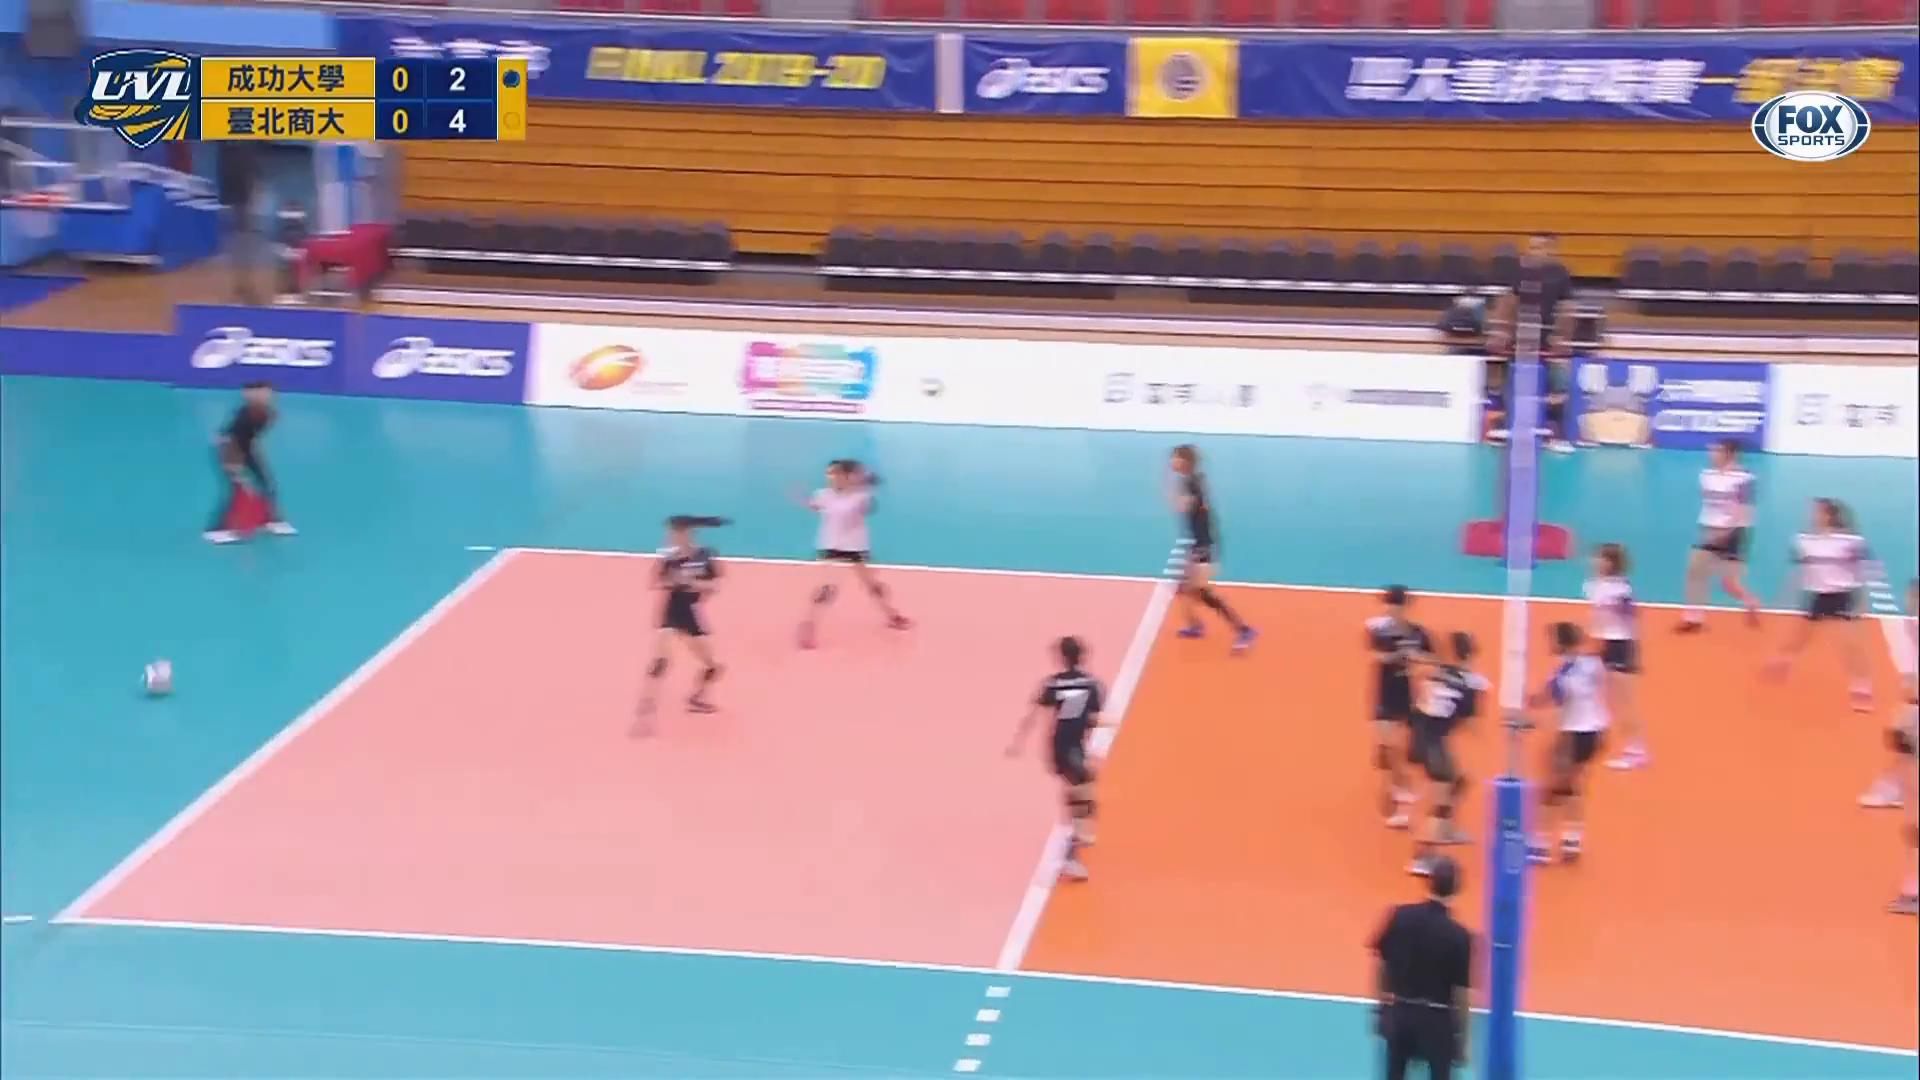
\includegraphics[width = 7cm]{picture/死球.jpg}
            \caption{、死球}
            \label{死球}
        \end{minipage}
    \end{figure}

    我們先記錄每個子影片的名稱、開始與結束時間在一個 csv 檔內,再使用 moviepy.editor 切割影片。
    
    記錄格式 : 局數\_A方比數\_B方比數, 開始時, 開始分, 開始秒, 結束時, 結束分, 結束秒(如表 \ref{紀錄格式示意圖} 所示)。

    \begin{table}[H]
        \centering
        \caption{、紀錄格式示意圖}
        \label{紀錄格式示意圖}
        \begin{tabular}{ccccccc}
            \hline
            1\_00\_00 & 0 & 5 & 35 & 0 & 5 & 46\\
            \hline
            1\_00\_02 & 0 & 6 & 18 & 0 & 6 & 22\\
            \hline
            1\_03\_03 & 0 & 7 & 39 & 0 & 7 & 43\\
            \hline
        \end{tabular}
    \end{table}

\begin{figure}[H]
\end{figure}

    程式碼:
    \begin{lstlisting}[language={Python}]
from moviepy.editor import *
import sys
import csv
with open('clips.csv', newline='') as csvfile:
    rows = csv.reader(csvfile)
    for row in rows:
        name=str(row[0])
        h1=int(row[1])
        m1=int(row[2])
        s1=int(row[3])
        h2=int(row[4])
        m2=int(row[5])
        s2=int(row[6])
        clip = VideoFileClip("video.mp4").subclip(t_start=(h1,m1,s1),t_end=(h2,m2,s2))
        clip.write_videofile(name+".mp4")
        print(name+" Finish!")
    \end{lstlisting}
    \item []
    \textbf{(二)標記資料集}
    
    \begin{itemize}
        \setlength\parindent{2em}
        \item []
        \textbf{1. 標記方式}

        我們使用 TrackNetV2 提供的 Labeling Tool 進行標記,使用方式如表 \ref{Labeling Tool 使用方式}:

        \begin{figure}[H]
            \centering
            \begin{minipage}[H]{0.48\textwidth}
                \begin{table}[H]
                    \centering
                    \caption{、Labeling Tool 使用方式}
                    \label{Labeling Tool 使用方式}
                    \begin{tabular}{cc}
                        \hline
                        \textbf{按鍵} & \textbf{功能}\\
                        \hline
                        滑鼠左鍵 & 點擊標記座標\\
                        \hline
                        W & 取消標記\\
                        \hline
                        D & 下一幀\\
                        \hline
                        E & 上一幀\\
                        \hline
                        S & 儲存為 .pkl 檔\\
                        \hline
                        Q & 離開\\
                        \hline
                    \end{tabular}
                \end{table}
            \end{minipage}
            \begin{minipage}[H]{0.48\textwidth}
                \centering
                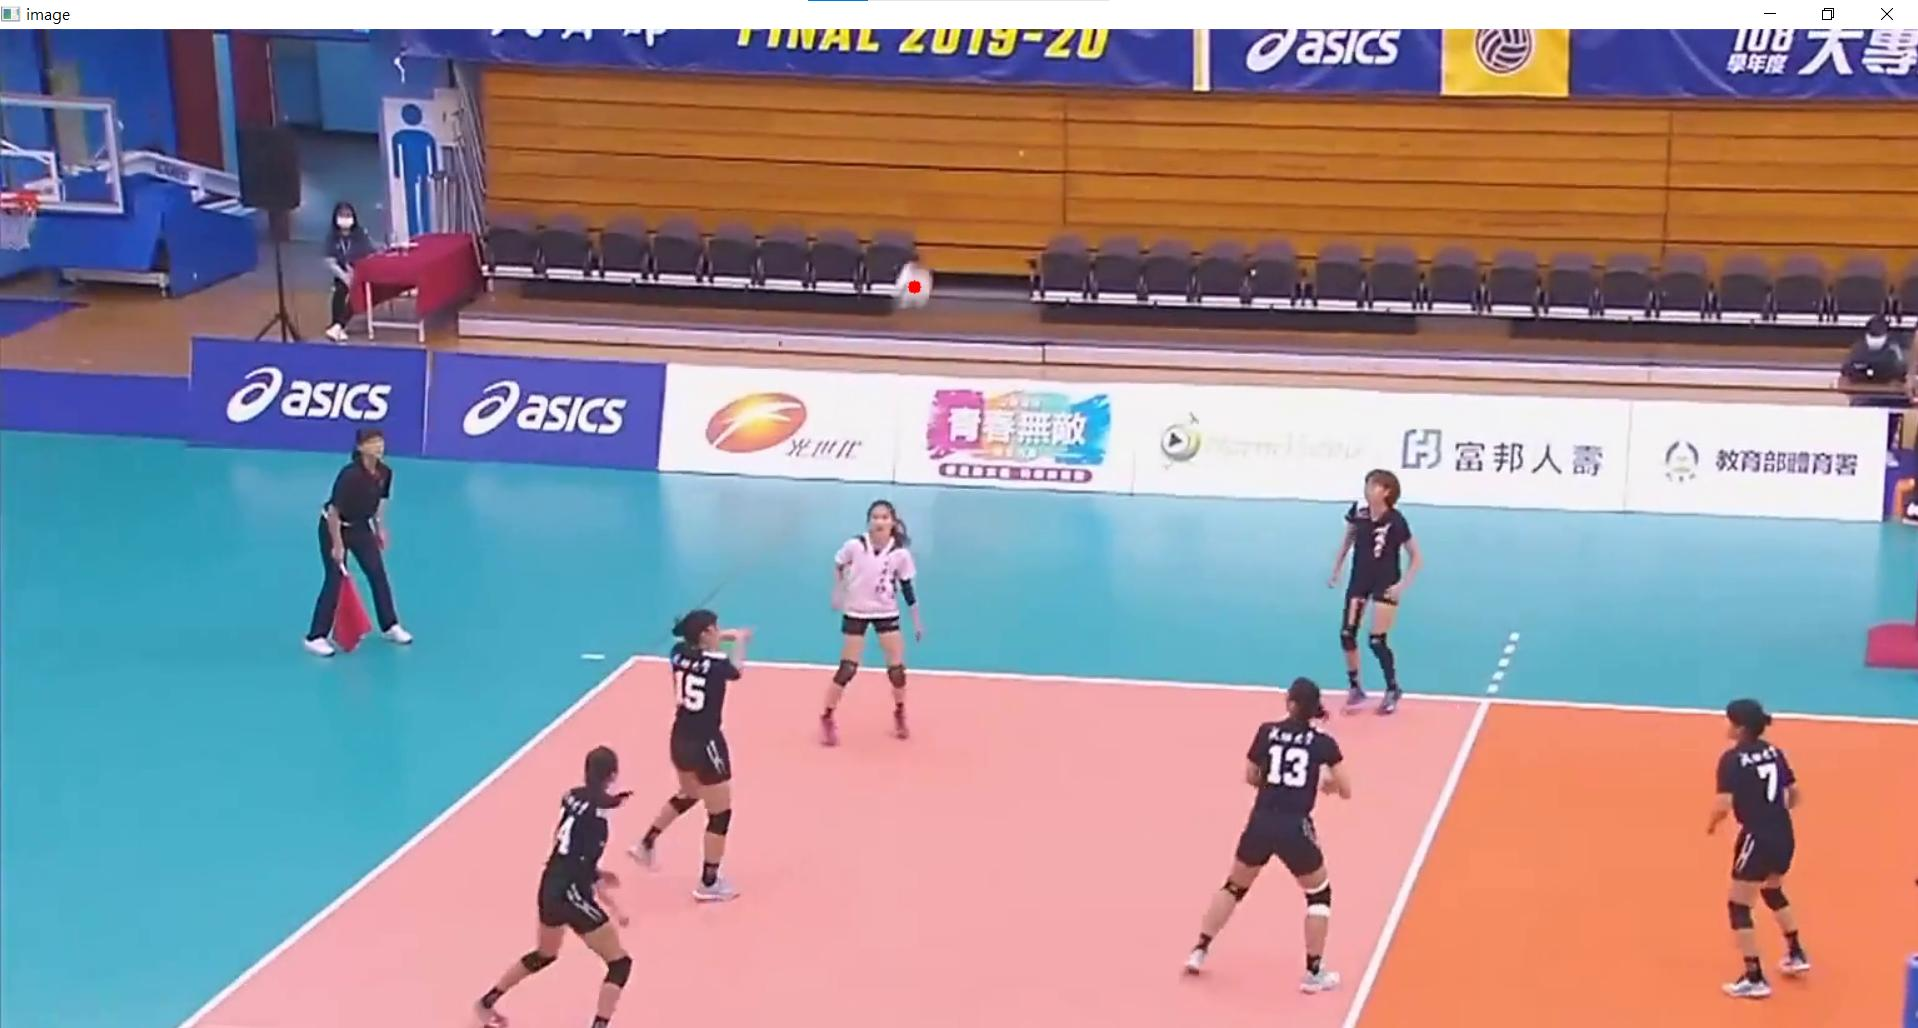
\includegraphics[width = 7cm]{picture/標記排球中心位置.jpg}
                \caption{、標記排球中心位置}
                \label{標記排球中心位置}
            \end{minipage}
        \end{figure}
        
        \item []
        \textbf{2. 輸出格式}

        標記完成後將輸出檔名為 *\_**\_**\_ball.csv 的檔案,格式如圖 \ref{標記輸出檔案格式}。

        \begin{figure}[H]
            \centering
            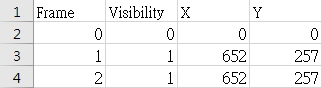
\includegraphics[width = 7cm]{picture/標記輸出檔案格式.jpg}
            \caption{、標記輸出檔案格式}
            \label{標記輸出檔案格式}
        \end{figure}

        Frame 表示此為第幾幀的資料,Visibility 表示是否可在圖片中看到排球(0 表無法,1 表可以),X 與 Y 則表示排球的座標。
    \end{itemize}
    
    \item []
    \textbf{(三)生成訓練數據}

    由標記資料與影片分割成的各幀圖片生成熱度圖等訓練數據,儲存為 .npy 檔。

    \item []
    \textbf{(四)訓練模型}

    使用上一步所生成的訓練資料進行訓練。

    \item []
    \textbf{(五)生成預測資料}
    
    我們由 108UVL 大專排球聯賽女一級冠軍賽擷取比賽片段做為測試資料運行 predict.py 生成預測資料,生成的兩個檔案分別為 *\_**\_**\_predict.mp4 及 *\_**\_**\_predict.csv ,前者是在影片上直接加上所預測的座標點,後者記錄了預測的可視性(是否可在圖片中看到排球)與座標。

    \item []
    \textbf{(六)效能評估}

    撰寫程式比對生成的預測資料與人工標記的資料。

    \begin{itemize}
        \setlength\parindent{2em}
        \item []
        \textbf{1. 分類方式}

        在影片中排球直徑大小約為 25 像素,所以我們將 TP 與 FP1的分界定為 10 像素。

        \begin{itemize}[itemindent = 2em]
            \item [(1)]\textbf{TP(True positives)}:預測的座標與人工標註的座標距離在 10 像素內
            \item [(2)]\textbf{TN(True negatives)}:無法看到球的樣本被正確識別為無法看到球
            \item [(3)]\textbf{FP1(False positives 1)}:預測的座標與人工標註的座標距離在 10 像素以上
            \item [(4)]\textbf{FP2(False positives 2)}:無法看到球的樣本被錯誤識別為可以看到球
            \item [(5)]\textbf{FN(False negatives)}:能看到球的樣本被錯誤識別為無法看到球
        \end{itemize}

        \item []
        \textbf{2. 評價指標計算}

        \begin{itemize}[itemindent = 2em]
            \item [(1)]\textbf{準確度(Accuracy)}:正確預測的樣本數占總樣本數的比例。
            $$Accuracy\ =\ \frac{TP+TN}{TP+TN+FP1+FP2+FN}$$
            \item [(2)]\textbf{精確度(Precision)}:預測為正樣本中真正為正樣本的比例。
            $$Precision\ =\ \frac{TP}{TP+FP1+FP2}$$
            \item [(3)]\textbf{召回率(Recall)}:被正確識別為正樣本的佔所有正樣本的比例。
            $$Recall\ =\ \frac{TP}{TP+FN}$$
            \item [(4)]\textbf{F1測量值(F1-measure)}:Precision 與 Recall 的調和平均。
            $$F1-measure\ =\ \frac{2\times Precision\times Recall}{Precision+Recall}$$
        \end{itemize}

        \item []
        \textbf{3. 程式碼}
        
        程式碼:
        
        \begin{lstlisting}[language={Python}]
import csv

def result(tp,tn,fp1,fp2,fn):
    accu = (tp+tn)/(tp+tn+fp1+fp2+fn)
    prec = tp/(tp+fp1+fp2)
    recall = tp/(tp+fn)
    f1 = 2*prec*recall/(prec+recall)
    print("TP :",tp,"\nTN :",tn,"\nFP1 :",fp1,"\nFP2 :",fp2,"\nFN :",fn)
    print("Accuracy :",accu)
    print("Precision :",prec)
    print("Recall :",recall)
    print("F1 measure :",f1)
    print()

tp_=0
fp1_=0
fp2_=0
tn_=0
fn_=0
contest_list=['1_03_02','1_04_02','1_04_03']
for name in contest_list:
    file = open(name+'_predict.csv')
    reader = csv.reader(file)
    predict = list(reader)
    file.close()
    file = open(name+'_ball.csv')
    reader = csv.reader(file)
    label = list(reader)
    file.close()
    del predict[0]
    del label[0]
    del label[1]
    del label[3]
    tp=0
    fp1=0
    fp2=0
    tn=0
    fn=0
    num = len(predict)
    for i in range(0,num):
        if (predict[i][1]=="0" and label[i][1]=="0"):
            tn+=1
        elif (predict[i][1]=="1" and label[i][1]=="0"):
            fp2+=1
        elif (predict[i][1]=="0" and label[i][1]=="1"):
            fn+=1
        else:
            sqdistance = (int(predict[i][2])-int(label[i][2]))**2+(int(predict[i][3])-int(label[i][3]))**2
            if (sqdistance <= 100):
                tp+=1
            else:
                fp1+=1
    print(name)
    result(tp,tn,fp1,fp2,fn)
    tp_+=tp
    fp1_+=fp1
    fp2_+=fp2
    tn_+=tn
    fn_+=fn
result(tp_,tn_,fp1_,fp2_,fn_)
        \end{lstlisting}
    \end{itemize}
\end{itemize}

\section{肆、研究結果}

由 108UVL 大專排球聯賽女一級冠軍賽擷取比賽片段做為測試資料,共擷取三段影片,全長 76 秒,共 2280 幀。(因為此模型是輸入三幀輸出一幀,所以每段影片的最前兩幀會作為輸入的資料而沒有預測結果,預測結果共 2274 幀)

\subsection{一、效能評估數據結果}

\begin{itemize}
    \item []\textbf{TP(True positives)}:預測的座標與人工標註的座標距離在 10 像素內(如圖 \ref{TP})
    \item []\textbf{TN(True negatives)}:無法看到球的樣本被正確識別為無法看到球(如圖 \ref{TN})
    \item []\textbf{FP1(False positives 1)}:預測的座標與人工標註的座標距離在 10 像素以上(如圖 \ref{FP1})
    \item []\textbf{FP2(False positives 2)}:無法看到球的樣本被錯誤識別為可以看到球(如圖 \ref{FP2})
    \item []\textbf{FN(False negatives)}:能看到球的樣本被錯誤識別為無法看到球(如圖 \ref{FN})
\end{itemize}

\begin{table}[H]
    \centering
    \caption{、數據結果}
    \label{數據結果}
    \begin{tabular}{ccccccccccc}
        \hline
        \textbf{比賽} & \textbf{TP} & \textbf{TN} & \textbf{FP1} & \textbf{FP2} & \textbf{FN} & \textbf{Total} & \textbf{Accuracy} & \textbf{Precision} & \textbf{Recall} & \textbf{F1-measure}\\
        \hline
        1\_03\_02 & 686 & 38 & 11 & 1 & 12 & 748 & 96.79\% & 98.28\% & 98.28\% & 98.28\%\\
        \hline
        1\_04\_02 & 570 & 69 & 23 & 3 & 23 & 688 & 92.88\% & 95.64\% & 96.12\% & 95.88\%\\
        \hline
        1\_04\_03 & 647 & 107 & 17 & 15 & 52 & 838 & 89.98\% & 95.29\% & 92.56\% & 93.90\%\\
        \hline
        總計 & 1903 & 214 & 51 & 19 & 87 & 2274 & 93.10\% & 96.45\% & 95.63\% & 96.04\%\\
        \hline
    \end{tabular}
\end{table}

統整三段影片的資料,我們的模型的評價指標數值如下:

\begin{itemize}
    \item []\textbf{準確度(Accuracy)}:93.10\%
    \item []\textbf{精確度(Precision)}:96.45\%
    \item []\textbf{召回率(Recall)}:95.63\%
    \item []\textbf{F1測量值(F1-measure)}:96.04\%
\end{itemize}

\subsection{二、影片結果}

觀看所生成的影片,可以看到多數時間此模型都能成功追蹤到球的位置,且預測的位置幾乎都位於球的正中央(包含球快速運動而產生殘影時),不過仍有少數幀無法追蹤到球。

以下為追蹤結果範例(亮黃色方框為人為加上,方便觀察到排球位置與預測結果(紅點處)的差異)。

\begin{figure}[H]
    \centering
    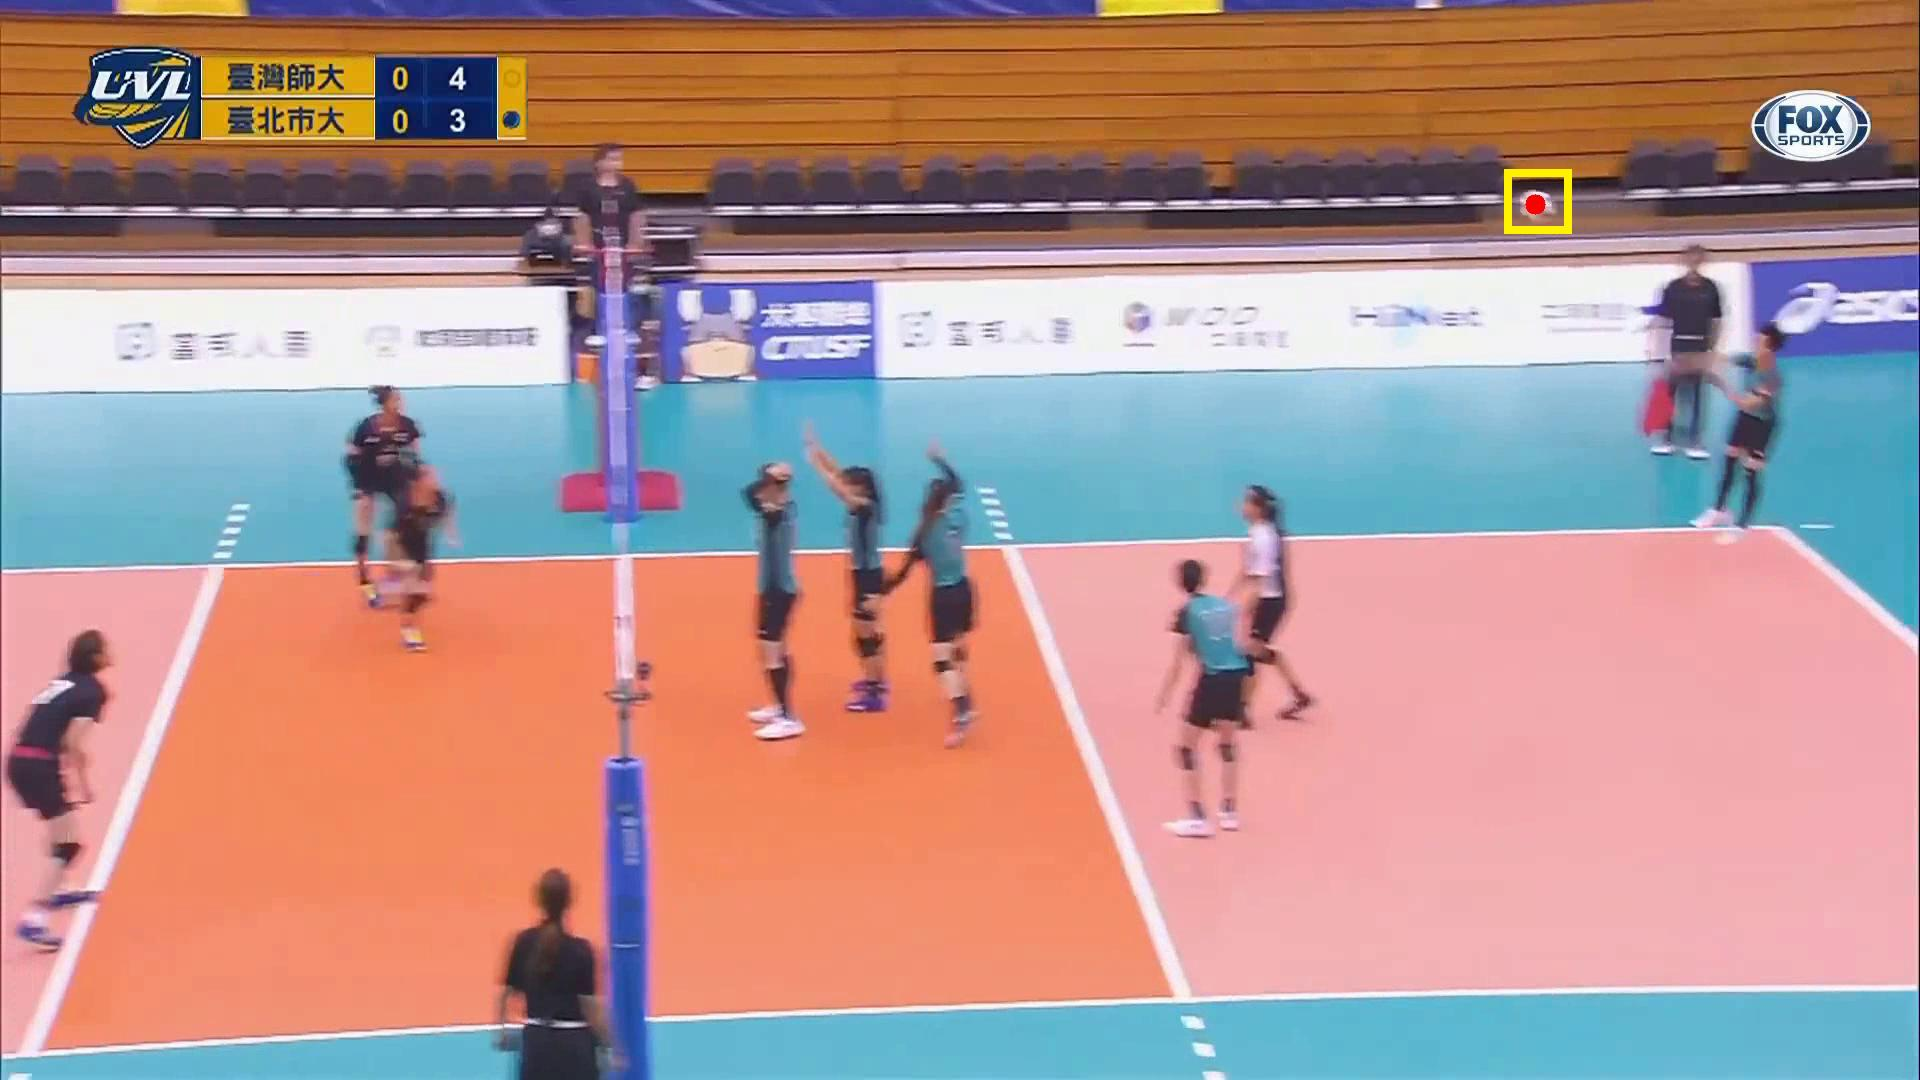
\includegraphics[width = 9cm]{picture/TP.jpg}
    \caption{、TP 範例(預測的座標與人工標註的座標距離在 10 像素內)}
    \label{TP}
\end{figure}

\begin{figure}[H]
    \centering
    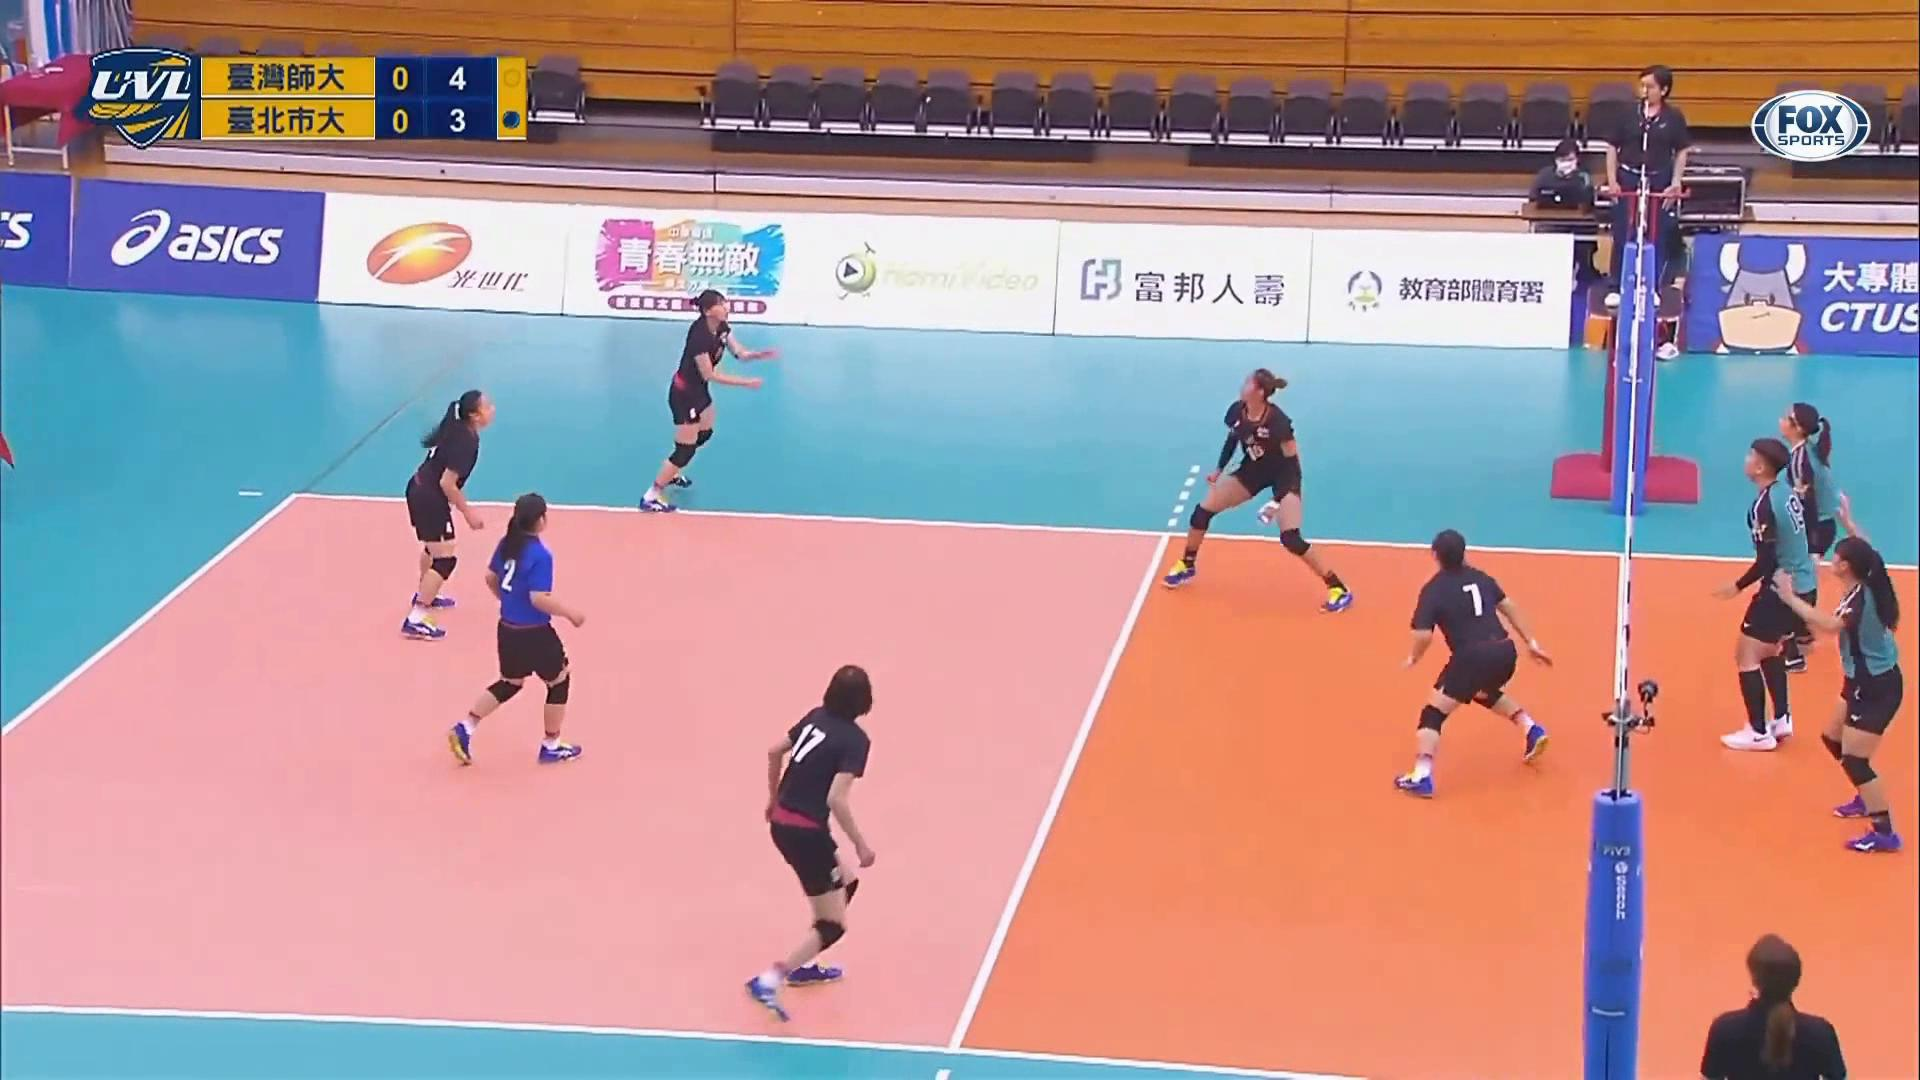
\includegraphics[width = 9cm]{picture/TN.jpg}
    \caption{、TN 範例(無法看到球的樣本被正確識別為無法看到球)}
    \label{TN}
\end{figure}

\begin{figure}[H]
    \centering
    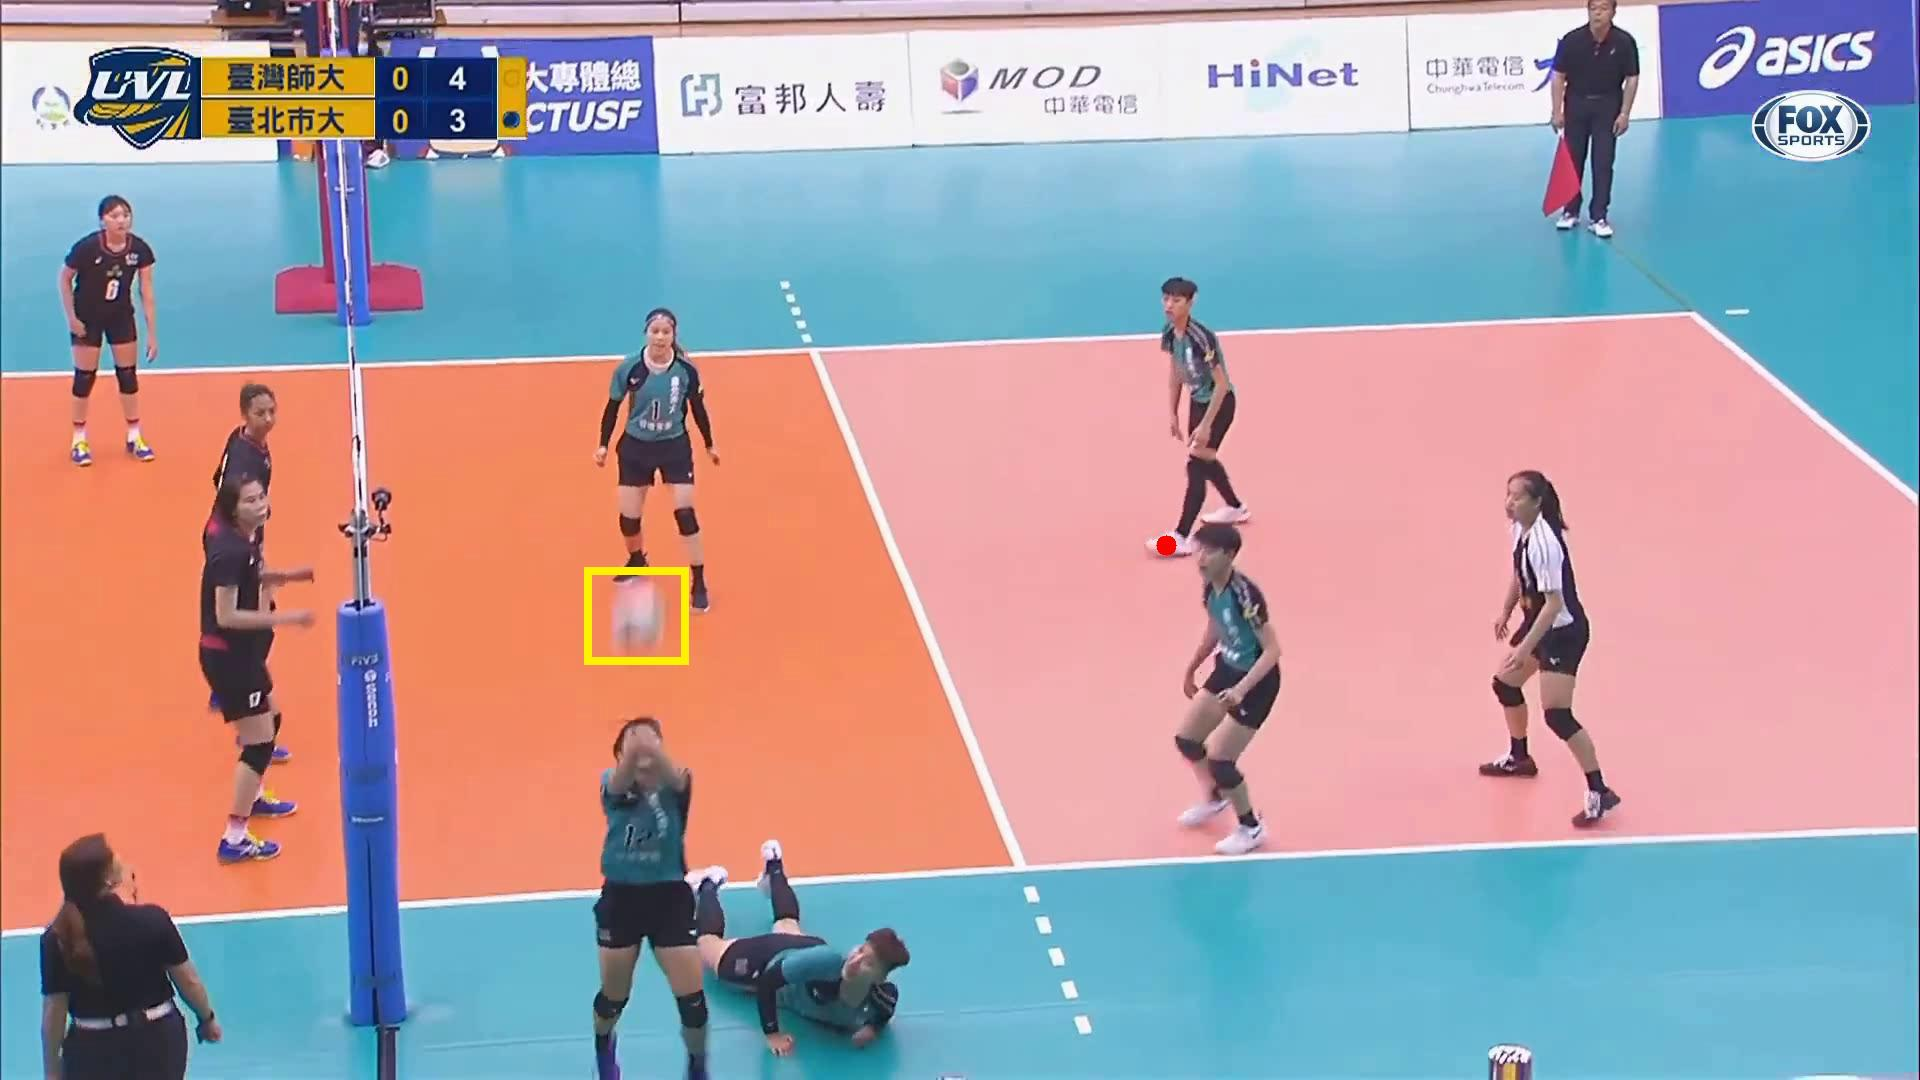
\includegraphics[width = 9cm]{picture/FP1.jpg}
    \caption{、FP1 範例(預測的座標與人工標註的座標距離在 10 像素以上)}
    \label{FP1}
\end{figure}

\begin{figure}[H]
    \centering
    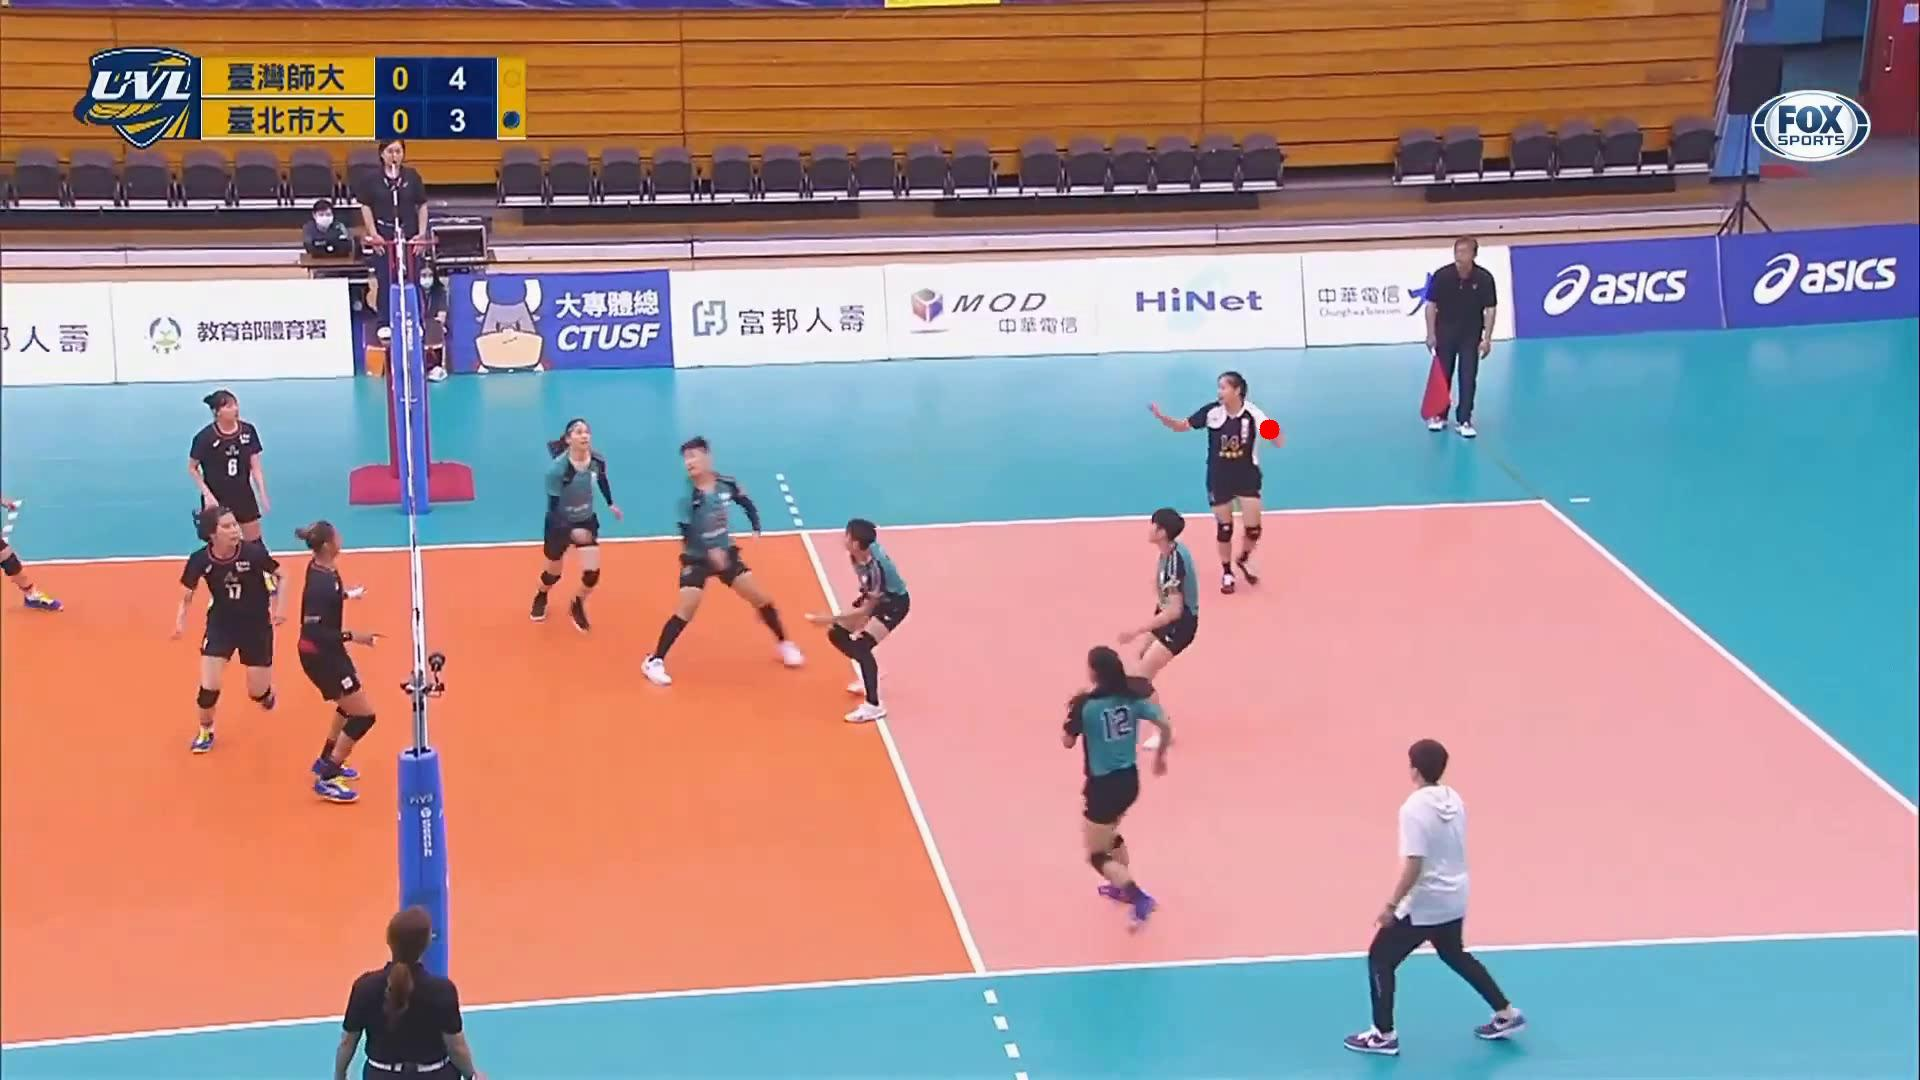
\includegraphics[width = 9cm]{picture/FP2.jpg}
    \caption{、FP2 範例(無法看到球的樣本被錯誤識別為可以看到球)}
    \label{FP2}
\end{figure}

\begin{figure}[H]
    \centering
    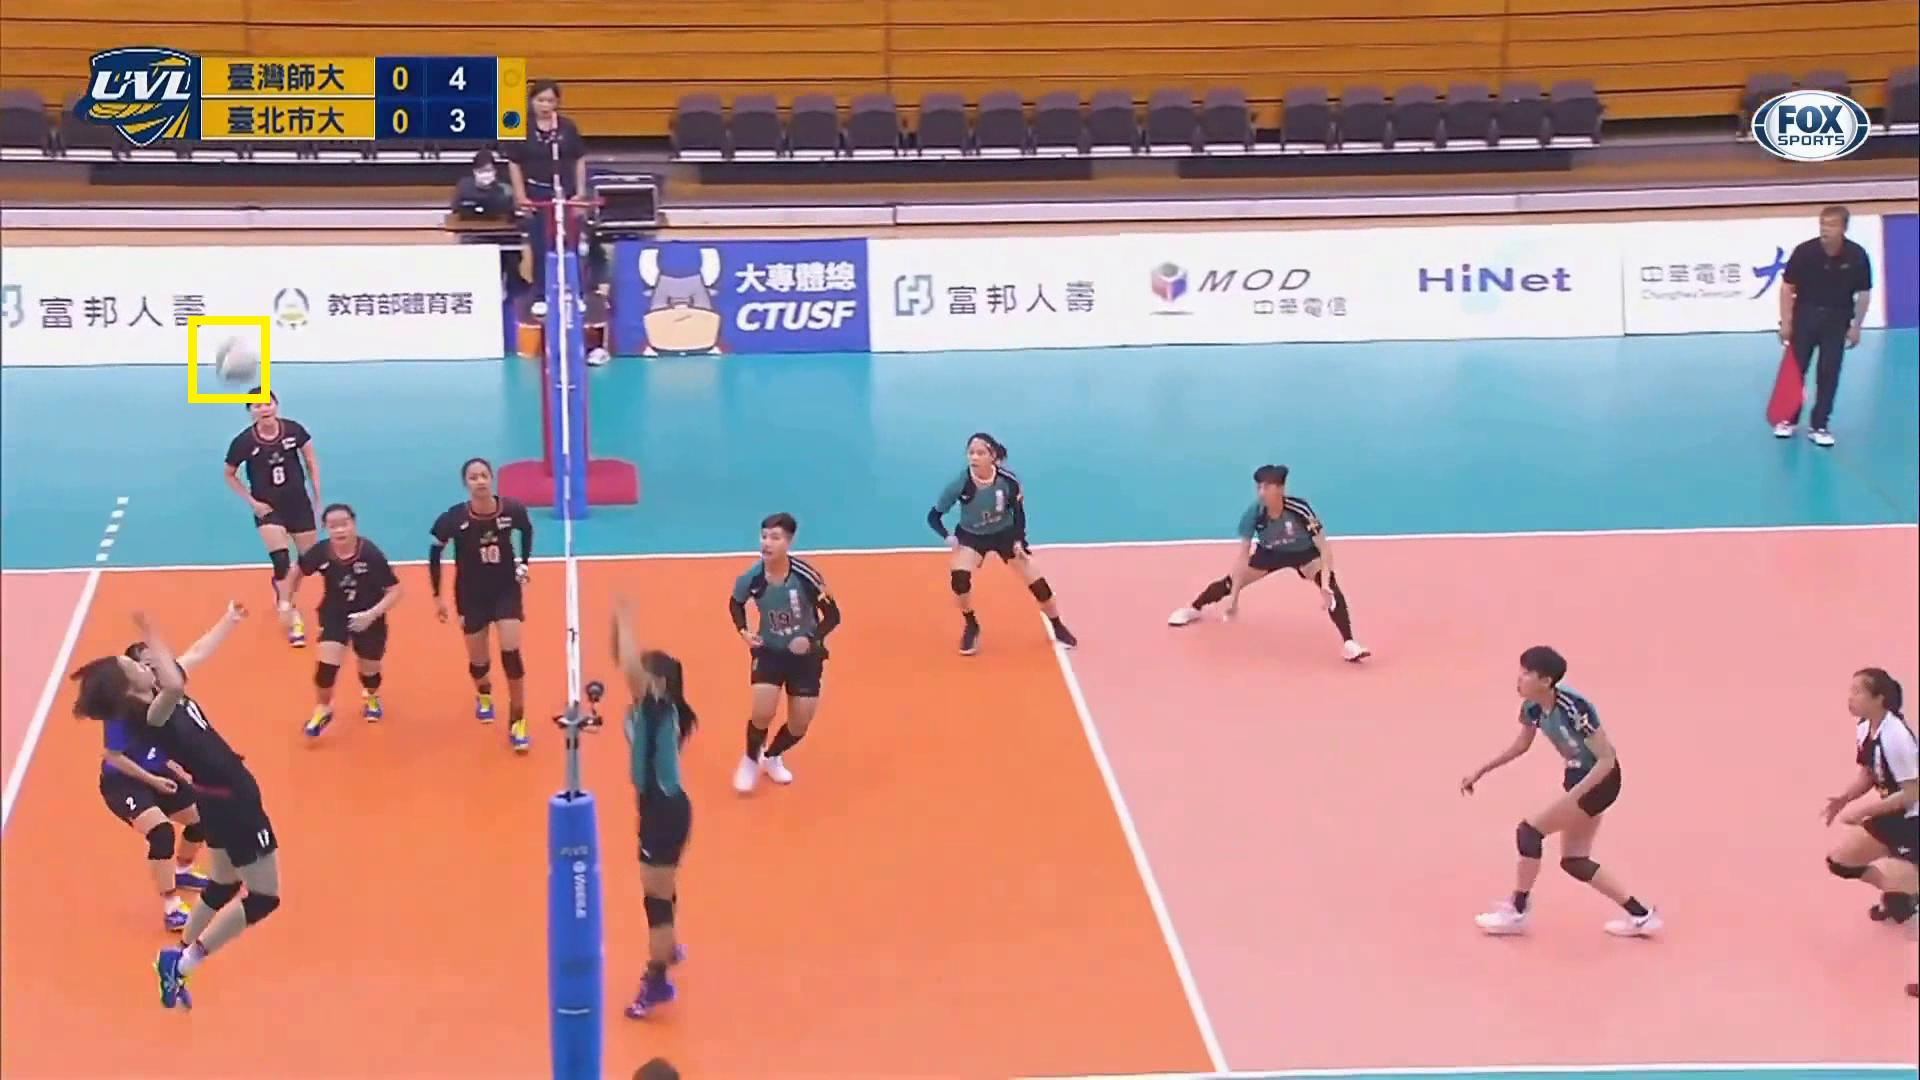
\includegraphics[width = 9cm]{picture/FN.jpg}
    \caption{、FN 範例(能看到球的樣本被錯誤識別為無法看到球)}
    \label{FN}
\end{figure}

\section{伍、討論}

\subsection{一、數據結果分析}

在追蹤錯誤的三個類別中,FN(87 幀)的數量最多而 FP2(19 幀)最少,由此得知我們的模型不容易在沒有球的畫面中偵測到球,但相對來說容易在有球的畫面中沒有偵測到球。

我們推測會沒有偵測到球的原因有以下幾點:排球與背景顏色相近、顏色相近的衣物等物體造成混淆、殘影造成形狀改變太大。這些問題甚至在人工標記訓練集時也會造成影響,而人工標記遇到此問題時的解決方法是往前後幀看,由前後幀推測排球可能所在位置再仔細看確認,所以我們猜想若是能讓模型學習到更多有關軌跡的部分可能可以解決這些問題,未來可以嘗試增加輸入圖片數量,例如由 3 張改為 5 張,使模型能學到更多軌跡的特徵。

\begin{figure}[H]
    \centering
    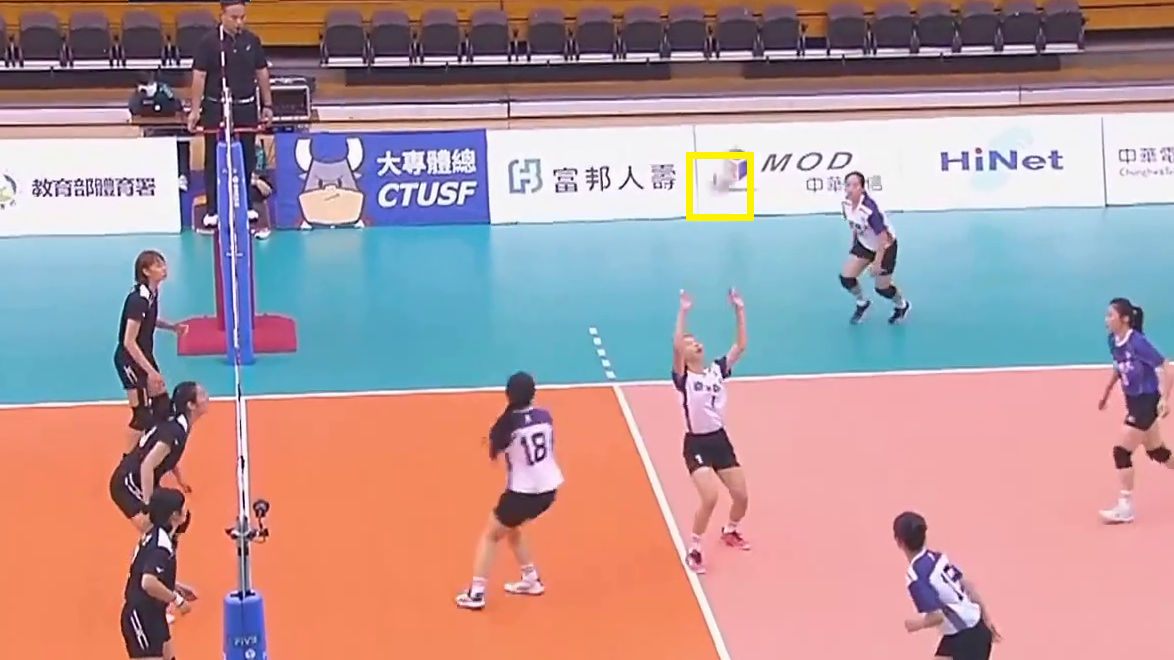
\includegraphics[width = 9cm]{picture/排球與背景顏色相近.jpg}
    \caption{、排球與背景顏色相近}
    \label{排球與背景顏色相近}
\end{figure}

\subsection{二、過度擬合問題}

過度擬合(overfitting)指的是過度緊密地去匹配特定資料集,以至於模型的泛化能力不佳(用其他測試資料去測試時效果不佳)。

我們的訓練資料皆來自於同一場比賽,場地與球的顏色皆相同(場地為藍色、橘色、粉紅色、橘色,排球為白色有黑色線條),測試資料也來自於相同場地的不同比賽,所以雖然我們測試出的模型表現不錯,但也有可能會發生過度擬合問題,在相同場地的表現很好不過換成其他顏色的場地或球表現就不佳,所以未來可以加入其他場地的比賽影片(如木頭地板、黃色球)訓練,減少過度擬合問題的發生,使模型在不同場地的比賽影片都能有效追蹤球的軌跡。

\subsection{三、錄影時鏡頭移動之影響}

在 TrackNet 及 TrackNetV2 所使用的網球及羽球影片皆為固定機位,模型在學習軌跡時不會被鏡頭的移動所干擾。我們使用的排球比賽影片是會隨著球的移動而轉動鏡頭,在錄影時鏡頭移動的影響下,球的軌跡不是自然生成的拋物線,因此有可能影響模型的表現。但根據我們的結果似乎影響不大,推測是因為鏡頭移動是跟隨球移動,是有規律性的,模型能夠學習到這個特徵。

\subsection{四、排球與羽球、網球差異}

球速方面,排球的球速較羽球及網球都低,以極限球速為例,排球 130 km/h 而羽球 493 km/h、網球 263 km/h。這會使得相機在拍攝排球比賽時出現的殘影較羽球及網球不嚴重,也就是拍攝到的形狀會比較接近球原本的形狀──圓形,模型在學習物體外型時可能會較容易。球速較慢也會使得每幀球移動的距離沒有那麼長。排球的體積也比網球和羽球大。

在人員方面,羽球和網球至多都只有 4 人,而排球有 12 人,這會使排球被人遮擋的機率比羽球和網球高,對結果造成影響。

\subsection{五、與 TrackNetV2 結果的差異與可能原因}

TrackNetV2 的結果中,Accuracy = 83.9\%, Precision = 90.7\%, Recall = 89.2\%;而我們的結果是 Accuracy = 93.1\%, Precision = 96.5\%, Recall = 95.6\%。推測這主要是因為上述提到的球速問題,羽球球速較快體積較小無法準確追蹤。除此之外,我們的測試資料和訓練資料皆來自同一場地,因此可能存在過度擬合的問題。

\subsection{六、未來展望}

綜上所述,我們認為未來可能的研究方向有以下幾點:

\begin{itemize}
    \setlength\parindent{2em}
    \item []
    \textbf{(一)加入更多不同場地數據}

    從不同比賽取得不同場地、排球顏色的影片資料進行訓練,在增加訓練資料的同時也能防止過度擬合問題的發生。

    \item []
    \textbf{(二)使用手機拍攝之影片實測}

    手機為目前民眾普遍擁有之拍攝工具,若我們訓練出的模型也能使用於手機拍攝之影片,而不只能應用於攝影機拍攝出的影片(如目前使用之訓練、測試集),此研究的實用性會更高。

    \item []
    \textbf{(三)精華片段擷取}

    由預測後的排球軌跡推測比賽的精華片段,例如殺球時軌跡通常為斜向由上而下且球速快,根據這類特徵自動從原本的比賽影片中擷取出精華片段。

    \item []
    \textbf{(四)分析戰略}
    
    除了球的軌跡外,同時追蹤球員及場地範圍,可能有助於分析戰略。

    \begin{itemize}
        \setlength\parindent{2em}
        \item []
        \textbf{1. 場地範圍}

        在場上找出幾個定位點(如球場端點),根據這些定位點訂出場地範圍。

        \item []
        \textbf{2. 球員追蹤}

        追蹤各個球員的動向。但此點應會較困難,因為在影片中不一定能一直看清各球員的背號,而且有時影片不會拍到所有球員或者球員重疊,在追蹤中斷後如何判斷並重新開始追蹤是需要解決的難點。
    \end{itemize}
\end{itemize}

\section{陸、結論}

我們訓練出的模型對於追蹤影片中排球的軌跡在相同場地下表現不錯,Accuracy = 93.1\%, Precision = 96.5\%, Recall = 95.6\%, F1-measure = 96.04\%。觀看所生成的影片時也可以看到大多數時間都有準確追蹤到排球的位置。

\section{柒、參考文獻資料}
\begin{itemize}[itemindent = 2em]
    \item [一、] 10 程式中(2021 年10 月6 日)。[Day 24] 機器學習- 不能忽視的過擬合與欠擬合。檢自:\url{https://ithelp.ithome.com.tw/articles/10278254}
    \item [二、]Brandon Da Silva (December 02, 2018). Playing Super Mario Bros with Proximal Policy Optimization. Retrieved from \url{https://brandinho.github.io/mario-ppo/}
    \item [三、]Chang-Chia-Chi (December 16, 2021). TrackNet-Badminton-Tracking-tensorflow2. Retrieved from \url{https://github.com/Chang-Chia-Chi/TrackNet-Badminton-Tracking-tensorflow2}
    \item [四、]Cinnamon AI Taiwan(June 5, 2019)。 深度學習:CNN原理。檢自:\url{https://cinnamonaitaiwan.medium.com/%E6%B7%B1%E5%BA%A6%E5%AD%B8%E7%BF%92-cnn%E5%8E%9F%E7%90%86-keras%E5%AF%A6%E7%8F%BE-432fd9ea4935}
    \item [五、]cs231n (June 15, 2021). Convolutional Neural Networks (CNNs / ConvNets). Retrieved from \url{https://brandinho.github.io/mario-ppo/}
    \item [六、]open-source / TrackNetV2 · GitLab (September 17, 2020). Retrieved from \url{https://nol.cs.nctu.edu.tw:234/open-source/TrackNetv2/tree/master}
    \item [七、]Shuttlecock Labeling Tool (May 18, 2021). Retrieved from \url{https://hackmd.io/@wCD9BlGyTByqPOqomNqWDA/HJKUBn-98}
    \item [八、]Nien-En Sun, Yu-Ching Lin, Shao-Ping Chuang, Tzu-Han Hsu, Dung-Ru Yu, Ho-Yi Chung, \& Tsì-Uí Ik (2020, December). \textit{TrackNetV2: Efficient Shuttlecock Tracking Network.} Paper presented at the 2020 International Conference on Pervasive Artificial Intelligence (ICPAI), Taipei, Taiwan.
    \item [九、]李謦伊(2020 年 9 月 29 日)。卷積神經網絡 Convolutional Neural Network (CNN)。檢自:\url{https://medium.com/ching-i/%E5%8D%B7%E7%A9%8D%E7%A5%9E%E7%B6%93%E7%B6%B2%E7%B5%A1-convolutional-neural-network-cnn-d7246d24ff3e}
    \item [十、]決賽::季軍賽::成功大學vs臺北商大::女一級 108UVL大專排球聯賽 網路直播(2020 年 4 月 19 日)。檢自:\url{https://www.youtube.com/watch?v=Vp4eJTpzX-E}
    \item [十一、]決賽::冠軍賽::臺灣師大vs臺北市大::女一級 108UVL大專排球聯賽 網路直播(2020 年 4 月 19 日)。檢自:\url{https://www.youtube.com/watch?v=3DjkhWQupkc&list=PLoy3tI0QCJ5OVpNZqf81YAwBESpM3yADv}
    \item [十二、]黃昱銓(2018)。利用深度學習熱度圖追蹤轉播影片中之網球(碩士論文)。檢自:\url{https://people.cs.nctu.edu.tw/~yi/TechReports/TrackNet.v1_Final_NOL.pdf}
    \item [十三、]鍾奉原(2020)。基於深度學習之網球軌跡影像分析(碩士論文)。檢自臺灣博碩士論文系統。(系統編號 108THU00396004)
\end{itemize}